%==============================================================================
\section{Introduction}
\label{section:Introduction}
%==============================================================================

As a quick tour through component--based software development using CCM Tools,
we implement a simple component that provides single interface to its clients.

\begin{figure}[htbp]
    \begin{center}
        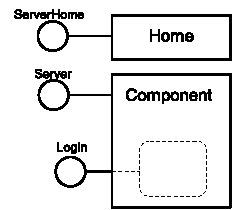
\includegraphics [width=5cm,angle=0] {figures/LoginComponentExample}
        \caption{ A simple component example.}
        \label{figure:SimpleComponentExample}
    \end{center}
\end{figure}

You will see how to define a simple component
(Fig.~\ref{figure:SimpleComponentExample}) in the CCM Tool's Interface
Definition Language (IDL) and how to use CCM Tools to generate code
in different programming languages.

\vspace{3mm}
The following sections are structured in form of CCM Tools use cases. Each use
case describes a usage scenario for a particular set of CCM Tools features. 
At the end of a use case, you will have a running component example.

\vspace{3mm}
This chapter contains a lot of CCM Tools stuff which will be described very
brief, never mind, you can find more exhaustive 	explanations in the related
manual chapters. 


\newpage


